\documentclass[tikz,border=4pt]{standalone}
\usepackage{amsmath}
\begin{document}
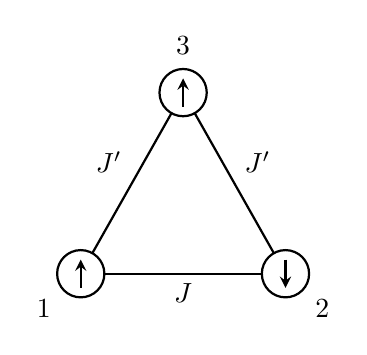
\begin{tikzpicture}[>=stealth, thick, scale=1.0]
  % Vertices of triangle
  \coordinate (V1) at (0, 0);
  \coordinate (V2) at (2.6, 0);
  \coordinate (V3) at (1.3, 2.3);

  % Edges
  \draw[thick] (V1) -- (V2) node[midway, below] {$J$};
  \draw[thick] (V2) -- (V3) node[midway, above right] {$J'$};
  \draw[thick] (V3) -- (V1) node[midway, above left] {$J'$};

  % Spin circles with arrows
  \filldraw[fill=white, draw=black, thick] (V1) circle (0.30);
  \draw[->, thick] (0, -0.18) -- (0, 0.18);
  \node[below left] at (-0.25, -0.20) {$1$};

  \filldraw[fill=white, draw=black, thick] (V2) circle (0.30);
  \draw[->, thick] (2.6, 0.18) -- (2.6, -0.18);
  \node[below right] at (2.85, -0.20) {$2$};

  \filldraw[fill=white, draw=black, thick] (V3) circle (0.30);
  \draw[->, thick] (1.3, 2.12) -- (1.3, 2.48);
  \node[above] at (1.3, 2.65) {$3$};
\end{tikzpicture}
\end{document}
